%----------------------------------------------------------------------------
\chapter{Hozzáférési szabályok kiértékelése}
%----------------------------------------------------------------------------
A hozzáférési szabályok több elemből állnak. A modell azon részeit, amelyekre a szabály vonatkozik, gráf mintákkal írjuk le. Ezek adják vissza az ún. asseteket, ezek lehetnek objektum (obj), attribútum (attr) vagy referencia (ref) modell elemek, ezekre adhatunk írási vagy olvasási jogosultságokat egyéni felhasználóknak vagy felhasználók egy csoportjának. Ezen kívül pedig prioritást is rendelhetünk a szabályokhoz, ezzel egy fontossági sorrendet felállítva közöttük.

\begin{figure}[H]
	\centering
	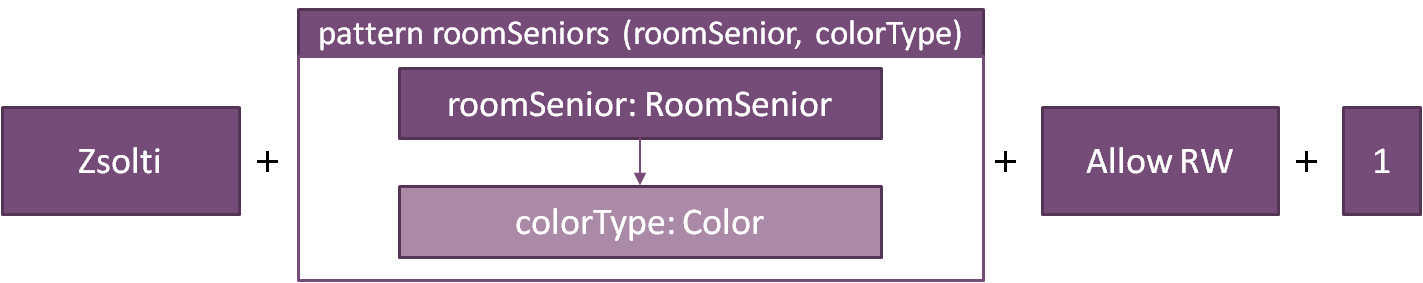
\includegraphics[width=150mm, keepaspectratio]{figures/rule.png}
	\caption{Egy szabály felépítése}
	\label{fig:rule}
\end{figure}

Vagyis a már említett szabályhoz a következőket kell meghatározunk: A Zsolti nevű felhasználónak az adott színű szobasenior objektumokra írási és olvasási engedélyt adunk, 1-es prioritással. Ezzel a gráfmintával egyelőre csak az összes szobaseniort tudjuk lekérdezni a színükkel együtt, később ezt a kört szűkíteni kell még, hogy csak a megfelelő színűek legyenek benne.

A szabályok érvényesítéséhez azokból először ún. judgementeket definiálunk. Egy judgement egy bizonyos asset elérhetőségére vagy módosítására tartalmaz engedélyt vagy tiltást, valamint ennek a prioritását. A hozzáférés-szabályozás ezen judgementek kiértékelése, összevetése alapján dönti el, hogy mely szabályok érvényesülnek. A lenti képen az előbb példaként felhozott szabály alapján létrejövő judgementek láthatók: a Timi és a Karesz nevű objektumok írhatók és olvashatók.

\begin{figure}[H]
	\centering
	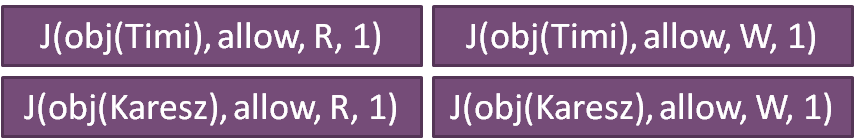
\includegraphics[width=150mm, keepaspectratio]{figures/judgement.png}
	\caption{A létrejövő judgementek}
	\label{fig:judgement}
\end{figure}

A már említett algoritmus - melynek célja a szabályok közötti ütközések feloldása - a megadott szabályok alapján definiált judgementek halmazát alakítja úgy, hogy a közöttük lévő konfliktusokat elemi konfliktusokra vezeti vissza, vagyis egy bizonyos assetre az egyik judgement engedélyez egy bizonyos műveletet, a másik tiltja azt. Ezek feloldásához először a judgementek prioritását veszi figyelembe, ha az megegyezik, akkor pedig az adott szabálynak az engedélyező vagy korlátozó tulajdonságát, amik az allow-t vagy a deny-t teszik dominánsabbá. Továbbá az olvasási/írási függőségek feloldására kibővíti az érvényre jutó judgementek listáját.
